%versi 2 (8-10-2016)-pppppppppppppp;
\chapter{Analisis}
\label{chap:analisis}
\setcounter{secnumdepth}{3}

\paragraph{} Pengumpulan data dalam skripsi ini dilakukan dengan cara studi pustaka untuk mempelajari cara pengembangan perangkat lunak menggunakan \textit{Framework} BlueTape yang berbasis CodeIgniter. Selain itu juga dipelajari \textit{library-library} pembantunya diantara lain : PHPExcel , Google OAuth dan ZurbFoundation. Tujuan studi pustaka ini untuk memahami secara rinci cara-cara untuk menambahkan layanan berbentuk modul ke dalam BlueTape dan membangun layanan tersebut menggunakan \textit{library-library} yang disebutkan sebelum ini.

\section{Analisis Sistem Kini(BlueTape)}
\paragraph{} Aplikasi \textit{Blue Tape} adalah perangkat lunak \textit{open source} sederhana yang memiliki tujuan utama untuk mengubah berbagai pekerjaan \textit{paper-based} di FTIS UNPAR menjadi \textit{paperless}. Selain itu perangkat lunak ini memiliki beberapa kegunaan lainnya seperti mengautentikasi mahasiswa dan staf UNPAR via OAuth 2.0 ke Google (layanan OAuth ke Google ini juga dapat digunakan untuk menentukan hak akses yang bisa dilihat dari email pengguna) dan \textit{Pilot Project} untuk permohonan transkrip ke Tata Usaha . Aplikasi ini merupakan aplikasi berbasis web dengan memanfaatkan \textit{Codeigniter} dan \textit{Zurb Foundation}. 
\newline
\begin{figure} [H]
	\centering  
	\frame{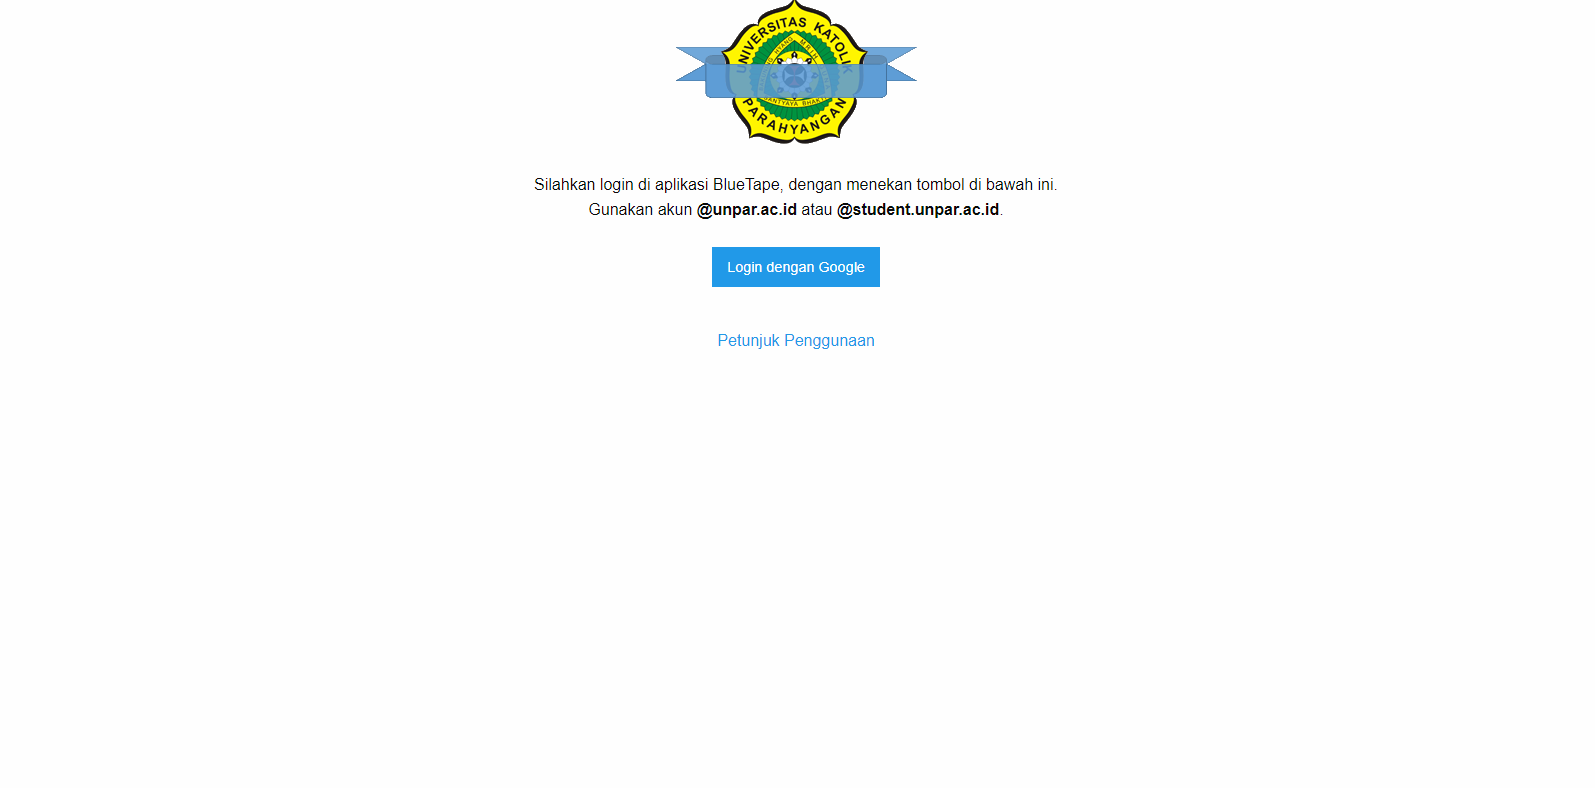
\includegraphics[scale=0.4]{halamanUtama.png}}
	\caption[Halaman Utama BlueTape Untuk Login dan Membuka Petunjuk Penggunaan]{Halaman Utama BlueTape Untuk Login dan Membuka Petunjuk Penggunaan} 
	\label{fig:flow-chart-CodeIgniter} 
\end{figure}
Perangkat lunak \textit{Blue Tape} ini didesain sebagai \textit{framework} yang terdiri dari beberapa layanan yang dipisahkan ke dalam modul-modul. Pemisahan layanan ke dalam modul-modul dibuat dengan tujuan agar pemeliharan perangkat lunak lebih mudah dan juga mempermudah cara untuk menambahkan layanan baru ke dalam BlueTape. Sudah ada layanan yang aktif di BlueTape saat ini yaitu \textit{Transcript Request / Manage} yang memiliki fungsi untuk melakukan permohonan serta pencetakan transkrip mahasiswa.

\subsubsection{\textit{Transcript Request / Manage}}
\paragraph{} Modul \textit{Transcript Request/Manage} merupakan salah satu dari dua modul yang sudah aktif di BlueTape ketika skripsi ini ditulis. Modul ini memiliki fungsi utama sebagai alat bagi mahasiswa untuk memohon pencetakan transkrip ke Tata Usaha dengan tampilan seperti di bawah ini :
\begin{figure} [H]
	\centering  
	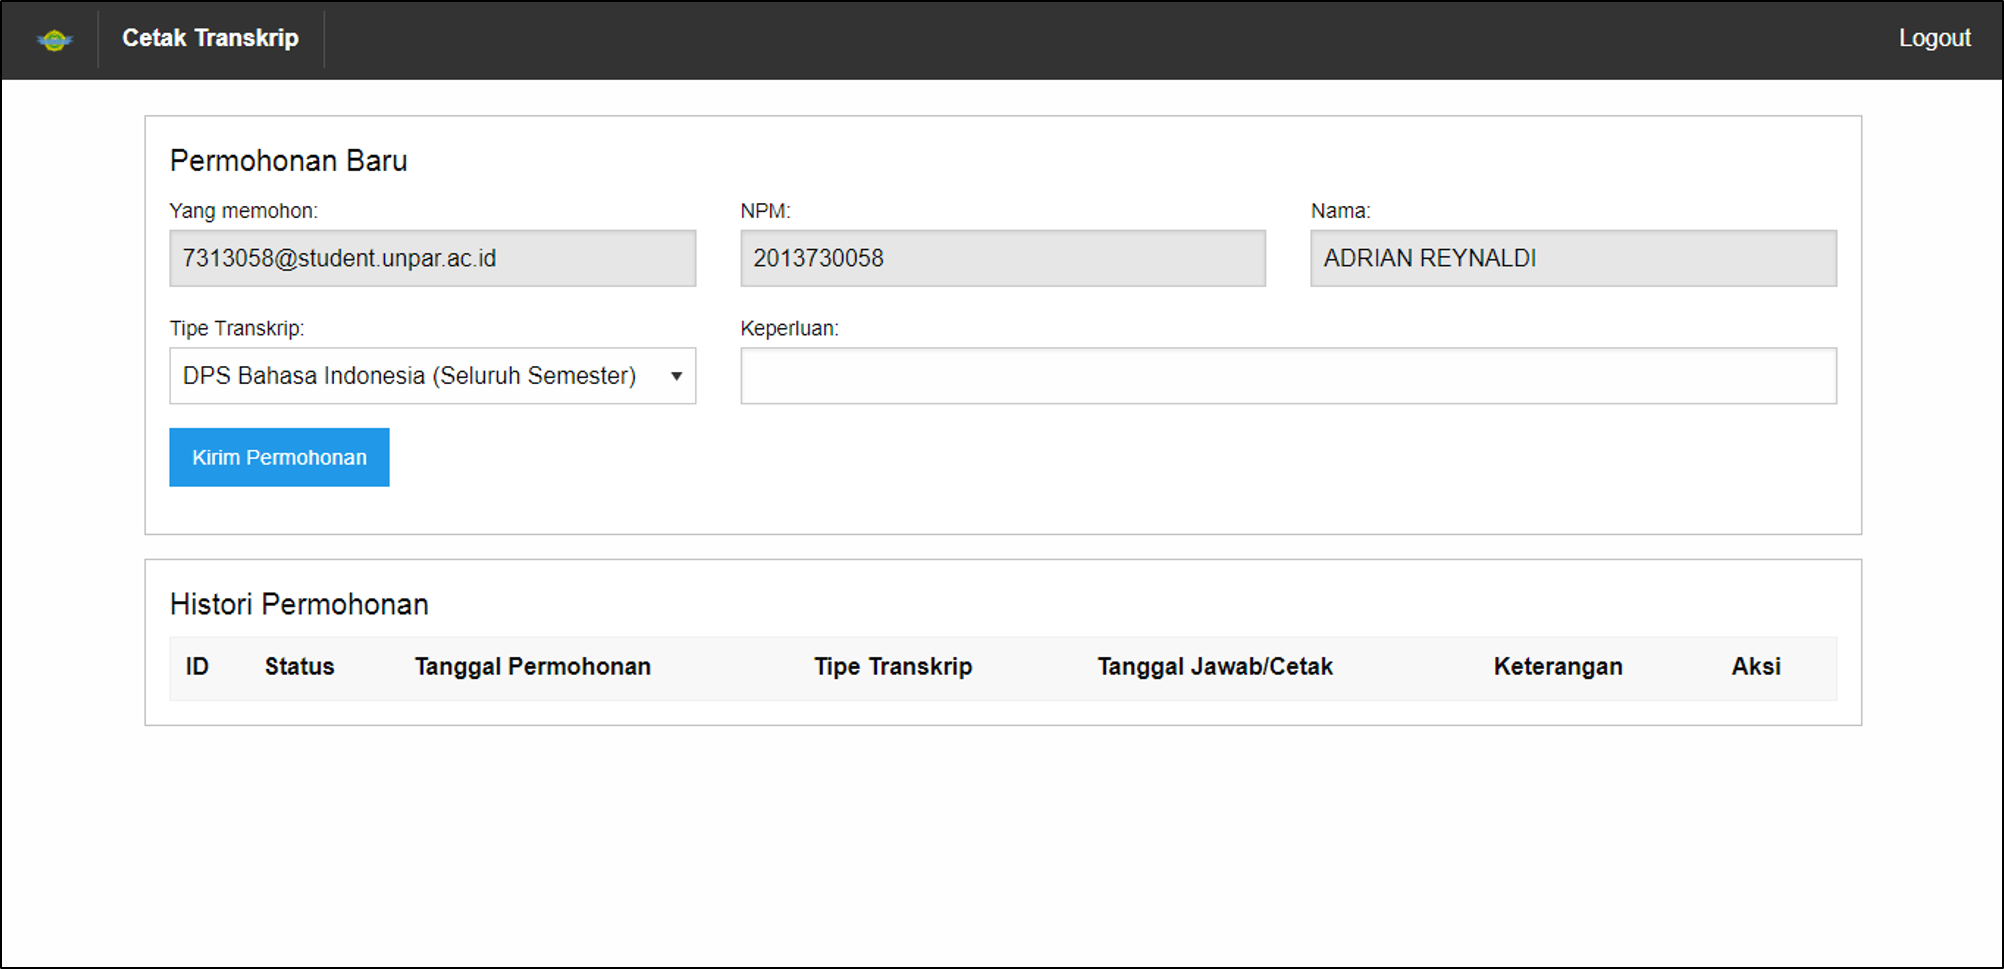
\includegraphics[scale=0.48]{cetakTranskrip.png}
	\caption[Tampilan Cetak Transkrip]{Tampilan Cetak Transkrip} 
	\label{fig:flow-chart-CodeIgniter} 
\end{figure}
\begin{figure} [H]
	\centering  
	\frame{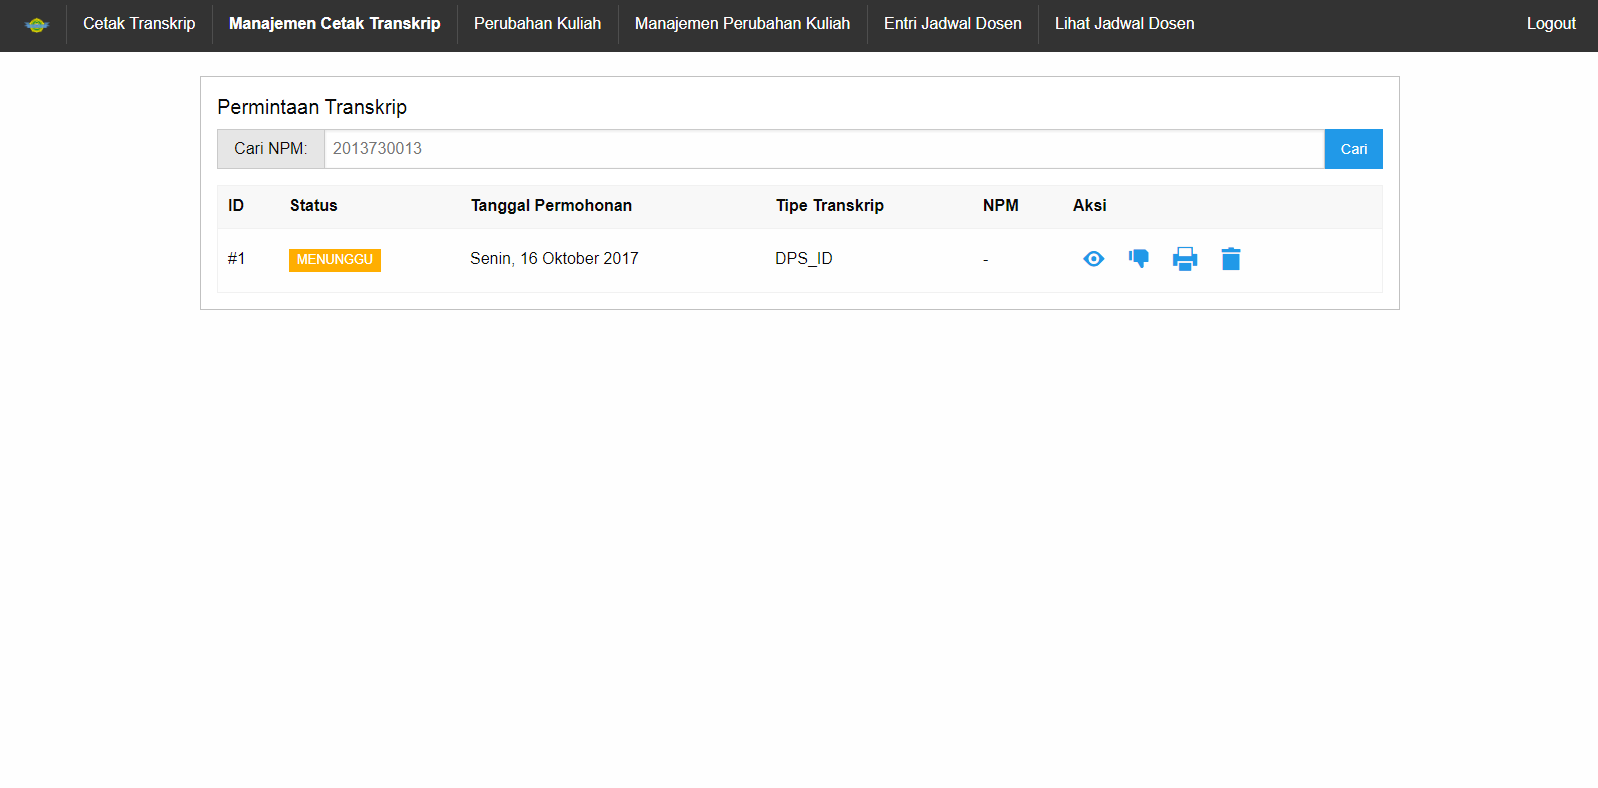
\includegraphics[scale=0.4]{manageTranskrip.png}}
	\caption[Tampilan Manajemen Transkrip]{Tampilan Manajemen Transkrip} 
	\label{fig:flow-chart-CodeIgniter} 
\end{figure}
Untuk memohon pencetakan transkrip pada halaman tersebut mahasiswa diperlukan untuk melakukan :
\begin{enumerate}
  \item Memilih salah satu dari 3 tipe transkrip yang ada. Ada 3 tipe transkrip: Daftar Perkembangan Studi (DPS) Bahasa Inggris, DPS Bahasa Indonesia dan Lembar Hasil Studi Semester Akhir.
  \item Lalu mahasiswa mengisi keterangan keperluan pencetakan transkrip di \textit{field} keperluan.
  \item Setelah kedua hal tersebut dipilih dan diisi , tekan tombol "Kirim Permohonan" untuk memohon pencetakan transkrip ke Tata Usaha.
\end{enumerate}
Tata usaha memiliki beberapa opsi untuk merespon permintaan yang sudah dikirim mahasiswa tadi :
\begin{enumerate}
	\item Melihat detail permintaan transkrip
	\item Menolak permintaan transkrip
	\item Mencetak detail permintaan transkrip
	\item Menghapus permintaan transkrip
\end{enumerate}

\subsubsection{Perubahan Kuliah}
\paragraph{} Perubahan kuliah adalah modul kedua yang sudah aktif di BlueTape. Modul ini berfungsi sebagai alat bagi mahasiswa untuk mengirimkan permintaan perubahan kuliah dari mahasiswa ke karyawan tata usaha. Selain itu karyawan tata usaha juga dapat menggunakan modul ini untuk mengatur permintaan-permintaan yang sudah dikirim dari mahasiswa tadi. 
\begin{figure} [H]
	\centering  
	\frame{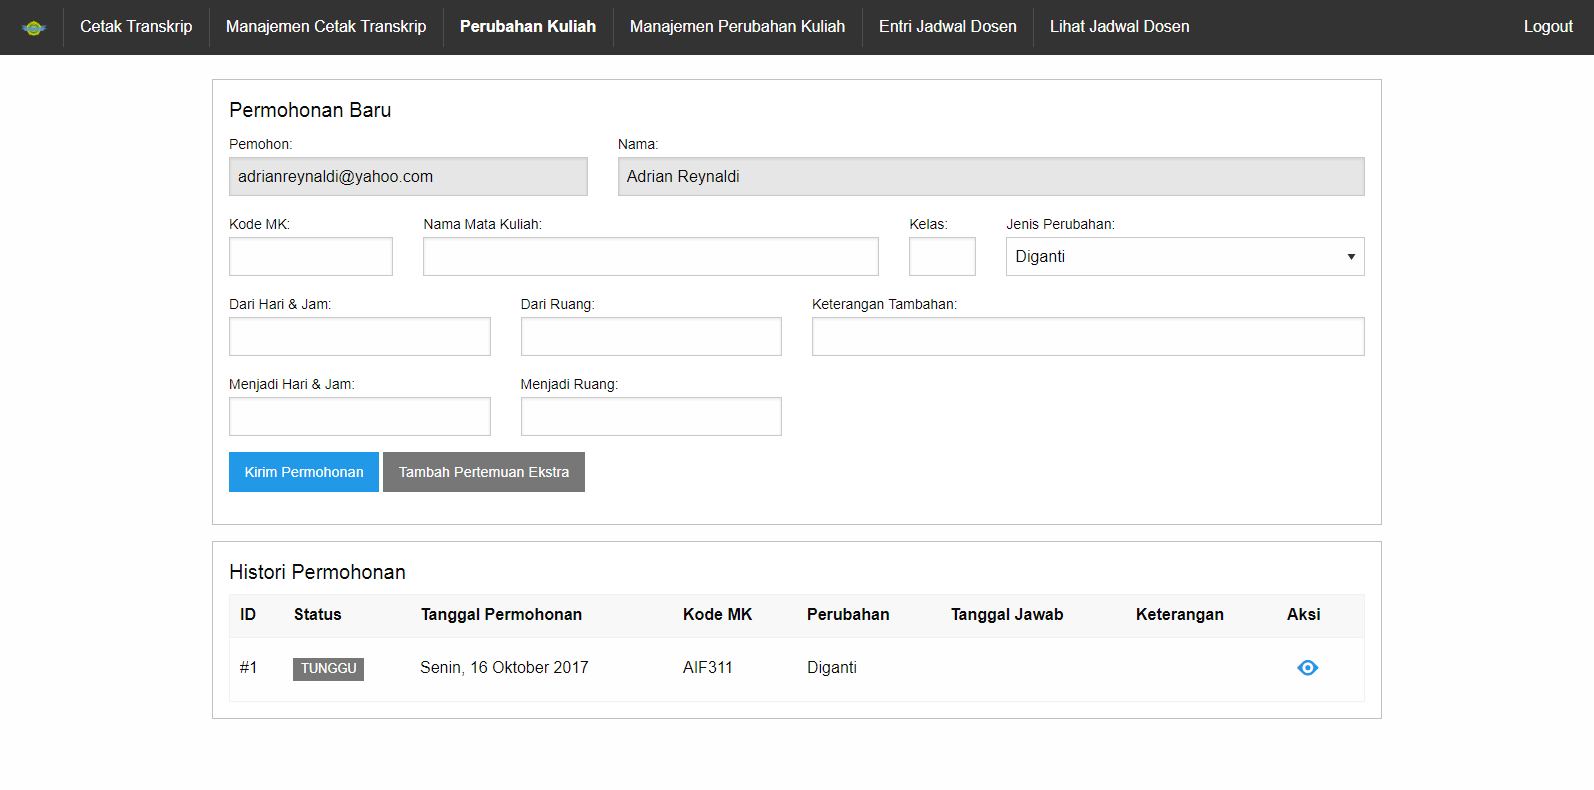
\includegraphics[scale=0.4]{perubahanKuliah.png}}
	\caption[Tampilan Menu Perubahan Kuliah]{Tampilan Menu Perubahan Kuliah} 
	\label{fig:flow-chart-CodeIgniter} 
\end{figure}
\begin{figure} [H]
	\centering  
	\frame{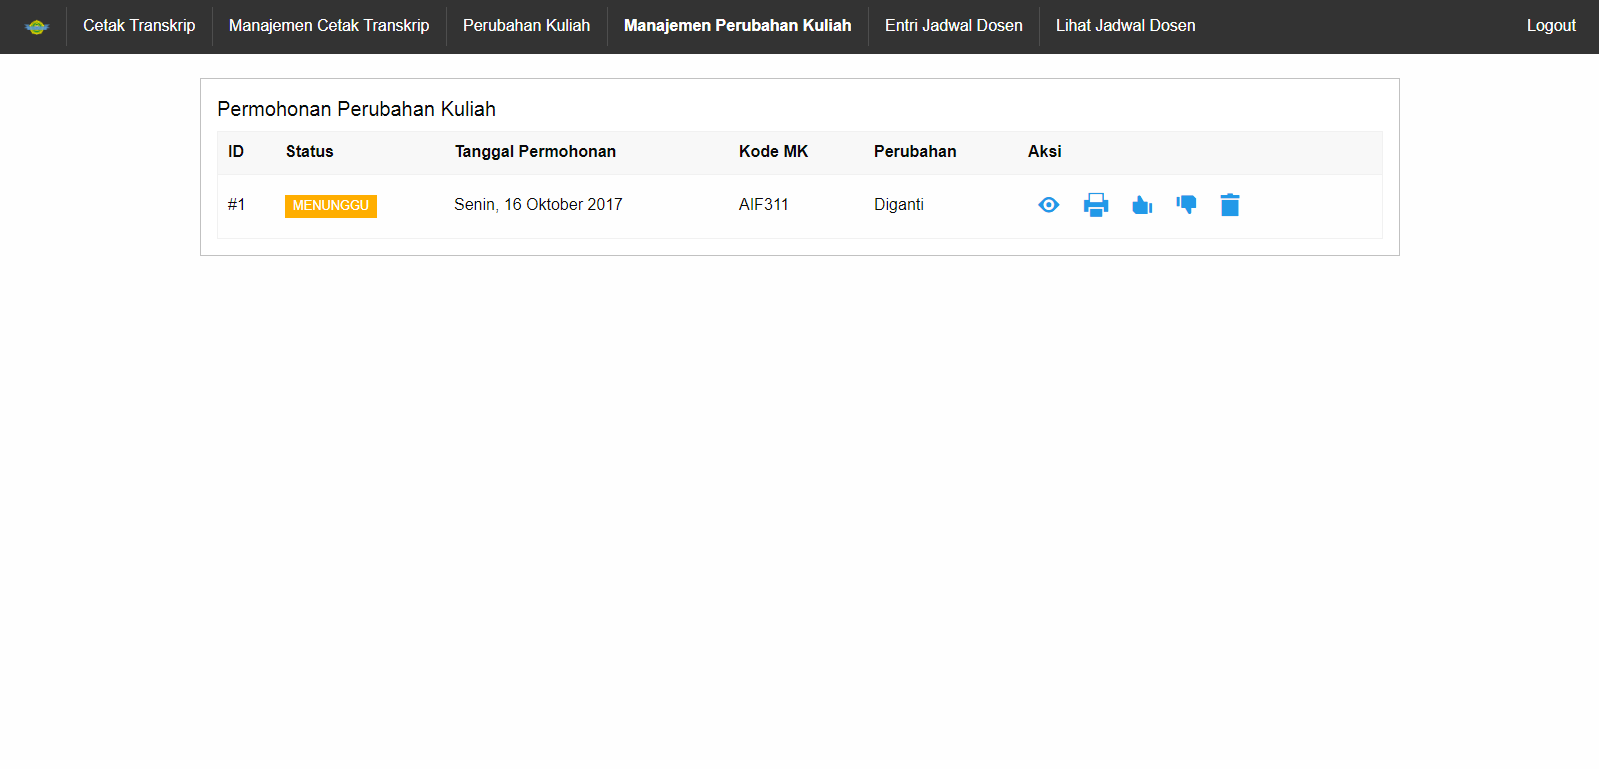
\includegraphics[scale=0.4]{managePerubahanKuliah.png}}
	\caption[Tampilan Menu Manajemen Perubahan Kuliah]{Tampilan Menu Manajemen Perubahan Kuliah} 
	\label{fig:flow-chart-CodeIgniter} 
\end{figure}
Untuk membuat permintaan perubahan kuliah, mahasiswa perlu mengisi setiap \textit{field} yang ada di menu. Setelah semua \textit{field} diisi, mahasiswa bisa memilih untuk mengirim permohonan atau tambah pertemuan.
\begin{itemize}
	\item Tombol "Kirim Permohonan" akan memeriksa apakah data yang sudah dimasukan sudah benar, bila sudah maka data permohonan akan dikrim ke server dan apabila ada yang masih salah maka sistem akan menandai bagian yang salah.
	
	\item Tombol "Tambah Pertemuan Ekstra" akan memunculkan 2 \textit{field} baru yaitu \textit{field} "Menjadi Hari dan jam" dan \textit{field} "Menjadi Ruang". Bila mahasiswa ingin mengirimkan permintaan penambahan pertemuan, tetap harus menekan tombol "Kirim Permohonan" setelah kedua \textit{field} yang baru tersebut juga diisi.
\end{itemize}
Di sisi tata usaha , modul ini memiliki fungsi untuk :
\begin{itemize}
	\item Menolak permintaan perubahan kuliah
	\item Menyetujui permintaan perubahan kuliah
	\item Mencetak detail perubahan kuliah
	\item Melihat detail perubahan kuliah
	\item Menghapus permintaan perubahan kuliah
\end{itemize}
  
\subsection{Pengguna Aplikasi}
Pada bagian ini akan dijelaskan pengelompokan tipe-tipe pengguna aplikasi BlueTape.

\subsubsection{Mahasiswa FTIS}
Mahasiswa FTIS adalah semua mahasiswa Fakultas Teknik Informasi dan Sains. Saat ini golongan Mahasiwa FTIS baru memiliki satu akses yaitu untuk memnita transkrip.


\subsubsection{Tata Usaha UNPAR}
Tata Usaha UNPAR adalah golongan pengguna yang bekerja sebagai staff tata usaha di Universitas Katolik Parahyangan. Di BlueTape, Tata Usaha UNPAR memilki akses fitur-fitur sebagai berikut :
\begin{itemize}
	\item Mengatur permintaan transkrip dari mahasiswa
	\item Mengatur permintaan perubahan kuliah 
\end{itemize}

\subsubsection{Staf UNPAR}
Staf UNPAR adalah para pekerja dan karyawan di Universitas Katolik Parahyangan. Untuk saat ini golongan staf UNPAR hanya memiliki akses fitur untuk meminta perubahan kuliah.

\subsubsection{Mahasiswa Informatika}
Mahasiswa Informatika adalah pengguna yang memiliki kepentingan untuk melihat jadwal-jadwal semua dosen Informatika. Dengan mengetahui jadwal dosen, maka mahasiswa dapat mengatur jadwal bimbingan atau konsultasi lainnya dengan dosen terkait secara lebih teratur. Di Bluetape, mahasiswa memiliki akses-akses pada fitur :
\begin{itemize}
	\item Melihat semua jadwal dosen Informatika
	\item Mengekspor semua jadwal dosen Informatika ke dalam tipe file .xls
	\item Meminta transkrip nilai
\end{itemize}

\subsubsection{Dosen Informatika}
Dosen merupakan pengguna yang akan memasukan jadwal-jadwalnya ke dalam BlueTape agar dapat dilihat mahasiswa. Dosen memilki akses pada fitur :
\begin{itemize}
	\item Memasukan jadwal ke dalam BlueTape
	\item Mengubah jadwal yang sudah dimasukan  
	\item Menghapus jadwal yang sudah dimasukan
	\item Melihat semua jadwal dosen , termasuk jadwal miliknya sendiri
	\item Mengeskpor semua jadwal dosen ke dalam tipe file .xls
\end{itemize}

\section{Analisis Sistem Usulan}

\section{Diagram Use Case}
\begin{figure} [H]
	\centering  
	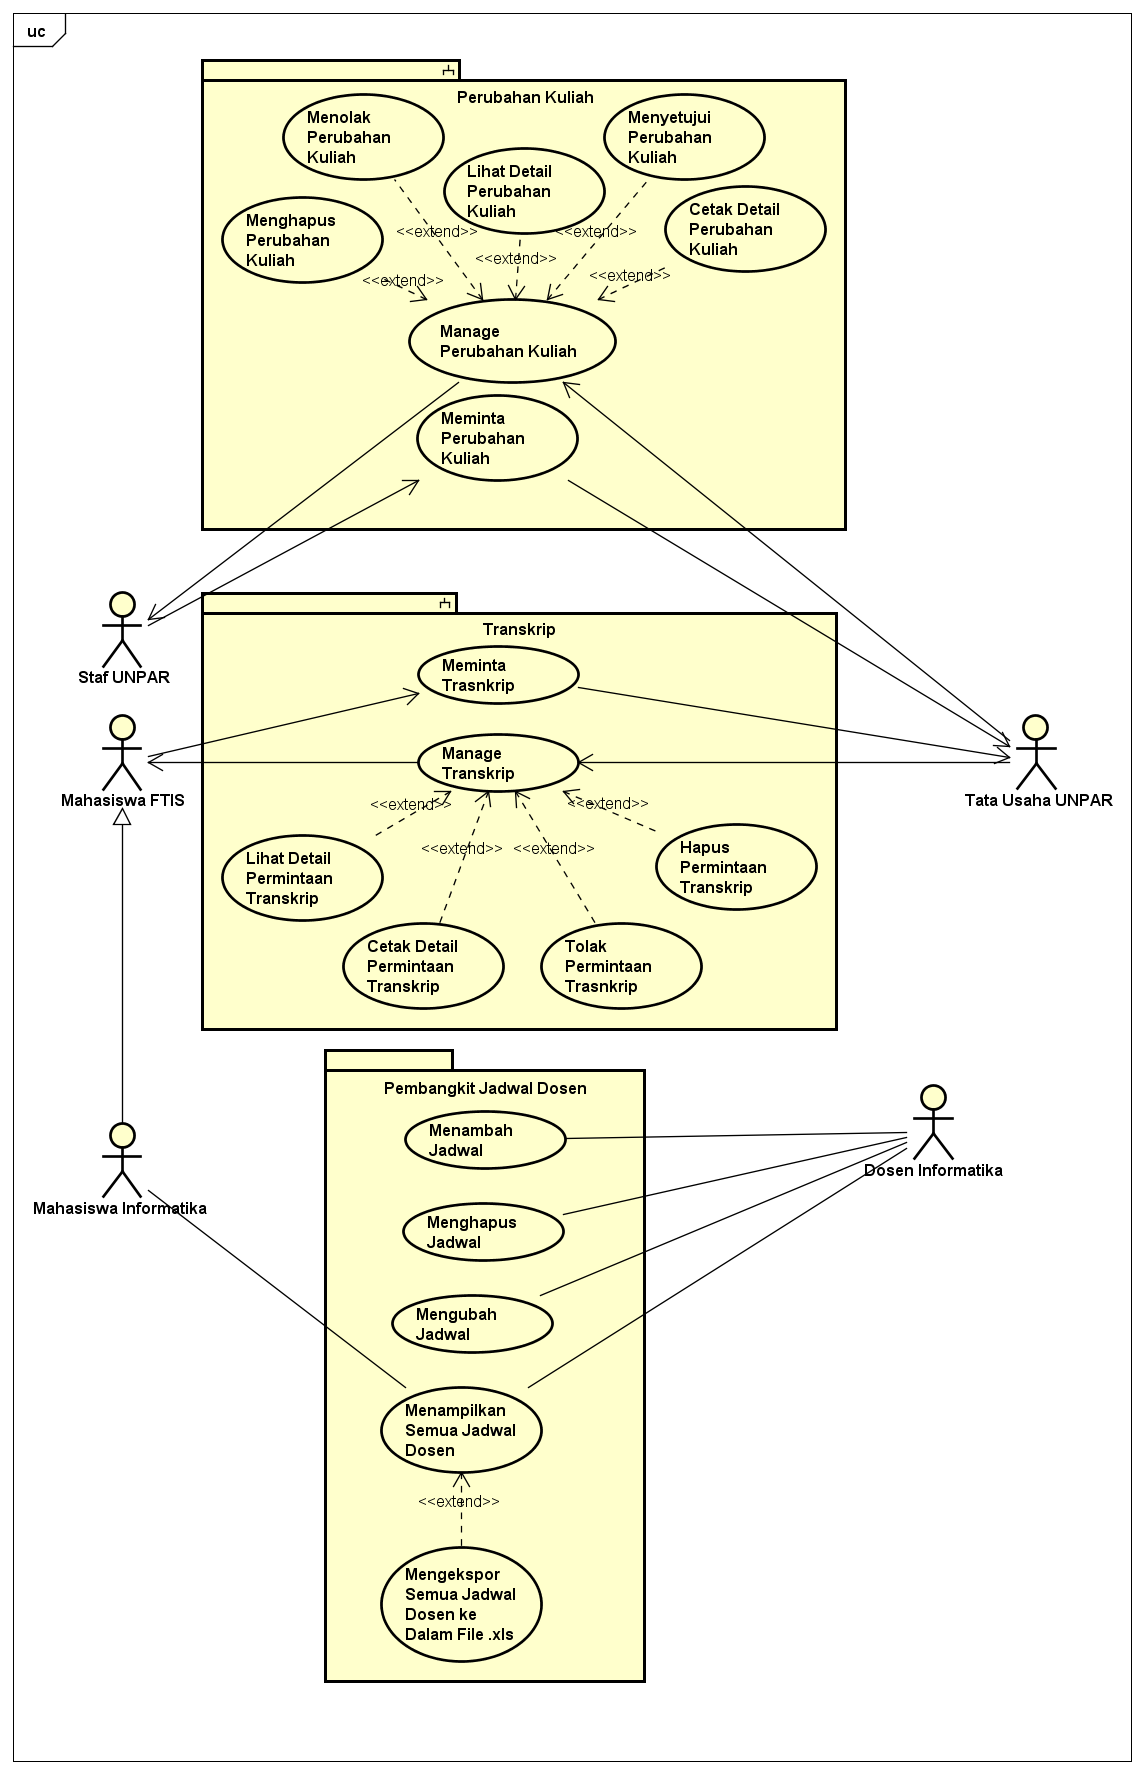
\includegraphics[scale=0.48]{useCaseDiagramSemua.png}
	\caption[Diagram Use Case]{Diagram Use Case} 
	\label{fig:flow-chart-CodeIgniter} 
\end{figure}
Berikut ini adalah penjelasan skenario dari diagram \textit{use case} di atas

\begin{enumerate}
	\item Skenario Meminta Perubahan Kuliah
	\begin{itemize}
		\item Aktor : Staf UNPAR, Tata Usaha UNPAR
		\item Skenario Normal
			\begin{enumerate}[1.]
				\item Staf UNPAR mengisi data-data yang diperlukan untuk melakukan perubahan kuliah
				\item Sistem mengirim data-data tersebut ke server 
				\item Tata Usaha menerima data yang dikirim oleh Staf UNPAR untuk diproses
			\end{enumerate}
		\item Skenario \textit{Exception}
			\begin{enumerate}[1.]
			 	\item Staf UNPAR memasukan data secara tidak lengkap
			 	\item Sistem menampilkan pesan eror karena data tidak lengkap
			\end{enumerate}
	\end{itemize}


	\item Skenario Melihat Detail Perubahan Kuliah
	\begin{itemize}
		\item Aktor : Tata Usaha UNPAR
		\item Skenario Normal
			\begin{enumerate}[1.]
				\item Aktor memilih data perubahan kuliah 
				\item Aktor memilih menu lihat detail
				\item Sistem menampilkan semua data-data permintaan mahasiswa dengan npm terkait 
			\end{enumerate}
	\end{itemize}
	
	\item Skenario Menolak Perubahan Kuliah 
	\begin{itemize}
		\item Aktor : Staf UNPAR, Tata Usaha UNPAR
		\item Skenario Normal
			\begin{enumerate}[1.]
				\item Tata Usaha UNPAR memilih data perubahan kuliah 
				\item Tata Usaha UNPAR memilih menu tolak perubahan kuliah
				\item Tata Usaha UNPAR mengisi data alasan penolakan
				\item Sistem mengirim pesan berisi alasan penolakan ke staf UNPAR
				\item Sistem menghapus permintaan perubahan kuliah dari \textit{database}
			\end{enumerate}
	\end{itemize}
	
	\item Skenario Menyetujui Perubahan Kuliah 
	\begin{itemize}
		\item Aktor : Staf UNPAR, Tata Usaha UNPAR
		\item Skenario Normal
			\begin{enumerate}[1.]
				\item Tata Usaha UNPAR memilih data perubahan kuliah 
				\item Tata Usaha UNPAR memilih menu tolak perubahan kuliah
				\item Tata Usaha UNPAR mengisi keterangan penyetujuan
				\item Sistem mengirim pesan berisi keterangan penyetujuan ke staf UNPAR
				\item Sistem menghapus permintaan perubahan kuliah dari \textit{database}
			\end{enumerate}
	\end{itemize}
	
	\item Skenario Menghapus Perubahan Kuliah 
	\begin{itemize}
		\item Aktor : Tata Usaha UNPAR
		\item Skenario Normal
			\begin{enumerate}[1.]
				\item Tata Usaha UNPAR memilih data perubahan kuliah 
				\item Tata Usaha UNPAR memilih menu hapus
				\item Sistem menghapus permintaan perubahan kuliah dari \textit{database}
			\end{enumerate}
	\end{itemize}

\item Skenario Cetak Detail Perubahan Kuliah 
	\begin{itemize}
		\item Aktor : Tata Usaha UNPAR
		\item Skenario Normal
			\begin{enumerate}[1.]
				\item Tata Usaha UNPAR memilih data perubahan kuliah 
				\item Tata Usaha UNPAR memilih menu cetak
				\item Sistem mencetak detail permintaan perubahan kuliah
			\end{enumerate}
	\end{itemize}
%=========================================================

	\item Skenario Meminta Transkrip
	\begin{itemize}
		\item Aktor : Mahasiswa FTIS
		\item Skenario Normal
			\begin{enumerate}[1.]
				\item Mahasiswa FTIS mengisi data keterangan dan tipe transkrip 
				\item Sistem menyimpan data-data tersebut ke server 
			\end{enumerate}
	\end{itemize}
	
	\item Skenario Lihat Detail Permintaan Transkrip
	\begin{itemize}
		\item Aktor : Tata Usaha UNPAR
		\item Skenario Normal
			\begin{enumerate}[1.]
				\item Tata Usaha UNPAR memilih data permintaan
				\item Tata Usaha UNPAR memilih menu lihat detail
				\item Sistem menampilkan detail data permintaan
			\end{enumerate}
	\end{itemize}
	
	\item Tolak Permintaan Transkrip
	\begin{itemize}
		\item Aktor : Tata Usaha UNPAR
		\item Skenario Normal
			\begin{enumerate}[1.]
				\item Tata Usaha UNPAR memilih data permintaan
				\item Tata Usaha UNPAR memilih menu tolak permintaan
				\item Sistem menampilkan menu keterangan penolakan
				\item Tata Usaha UNPAR mengisi data keterangan penolakan
				\item Sistem mengirim pesan berisi keterangan penolakan ke Mahasiswa FTIS.
			\end{enumerate}
	\end{itemize}
	
	\item Hapus Permintaan Transkrip
	\begin{itemize}
		\item Aktor : Tata Usaha UNPAR
		\item Skenario Normal
			\begin{enumerate}[1.]
				\item Tata Usaha UNPAR memilih data permintaan
				\item Tata Usaha UNPAR memilih menu hapus
				\item Sistem menampilkan pesan konfirmasi
				\item Tata Usaha UNPAR mengkonfirmasi penghapusan
				\item Sistem menghapus data permintaan dari \textit{database}
			\end{enumerate}
	\end{itemize}

%==========================================================
	\item Skenario Menambah Jadwal
	\begin{itemize}
		\item Aktor : Dosen Informatika
		\item Skenario Normal
			\begin{enumerate}[1.]
				\item Dosen Informatika mengisi data jadwal
				\item Sistem menyimpan data jadwal tersebut ke dalam \textit{database}
			\end{enumerate}
	\end{itemize}

	\item Skenario Mengubah Jadwal
	\begin{itemize}
		\item Aktor : Dosen Informatika
		\item Skenario Normal
			\begin{enumerate}[1.]
				\item Dosen Informatika memilih jadwal yang akan diubah
				\item Sistem menampilkan menu pengubahan berisi data jadwal yang dipilih tadi
				\item Dosen Informatika mengubah data-data yang ingin diubah
				\item Sistem menyimpan hasil perubahan ke dalam database
			\end{enumerate}
	\end{itemize}


	\item Skenario Menghapus Jadwal
	\begin{itemize}
		\item Aktor : Dosen Informatika
		\item Skenario Normal
			\begin{enumerate}[1.]
				\item Dosen Informatika memilih jadwal yang akan dihapus
				\item Sistem menampilkan menu pengubahan berisi data jadwal yang dipilih
				\item Dosen Informatika menekan tombol hapus
				\item Sistem menghapus data jadwal tersebut yang ada di database
			\end{enumerate}
	\end{itemize}

	\item Skenario Menampilkan Semua Jadwal Dosen
	\begin{itemize}
		\item Aktor : Mahasiswa Informatika , Dosen Informatika
		\item Skenario Normal
			\begin{enumerate}[1.]
				\item Aktor memilih menu lihat jadwal dosen
				\item Sistem memuat semua data jadwal-jadwal dari \textit{database}
				\item Sistem mengelompokan setiap jadwal berdasarkan pemiliknya
				\item Sistem membuat tab-tab yang merepresentasikan setiap dosen yang sudah menyimpan jadwal ke dalam database
				\item Sistem memasukan jadwal-jadwal ke dalam tab-tab sesuai nama pemiliknya.
			\end{enumerate}
	\end{itemize}
	

	\item Skenario Mengekspor Semua Jadwal Dosen ke Dalam File .xls
	\begin{itemize}
		\item Aktor : Mahasiswa Informatika , Dosen Informatika
		\item Skenario Normal
			\begin{enumerate}[1.]
				\item Aktor memilih menu lihat jadwal dosen
				\item Sistem memuat semua data jadwal-jadwal dari \textit{database}
				\item Sistem mengelompokan setiap jadwal berdasarkan pemiliknya
				\item Sistem membuat tab-tab yang merepresentasikan setiap dosen yang sudah menyimpan jadwal ke dalam database
				\item Sistem memasukan jadwal-jadwal ke dalam tab-tab sesuai nama pemiliknya.
				\item Aktor menekan tombol ekspor
				\item Sistem mengkonversi semua data jadwal dari bentuk php ke dalam bentuk \textit{spreadsheet} .xls
				\item Sistem menampilkan menu pemilihan lokasi penyimpanan \textit{file} .xls
				\item Aktor menekan tombol simpan
				\item Sistem menyimpan file .xls tersebut di lokasi yang sudah dipilih oleh aktor.
			\end{enumerate}
		\item Skenario Exception
			\begin{enumerate}[1.]
				\item Aktor memilih menu lihat jadwal dosen
				\item Sistem memuat semua data jadwal-jadwal dari \textit{database}
				\item Sistem tidak menerima data apapun dari \textit{database}
				\item Sistem men-\textit{disable} tombol ekspor
			\end{enumerate}
	\end{itemize}
\end{enumerate}